% Báo cáo tiến độ: baseline06.ipynb (A), baseline06v3.ipynb (B), đối chiếu bài shape vector.
% Biên dịch: XeLaTeX hoặc pdfLaTeX (Overleaf). Cần thư mục figures/ đặt cạnh file này.
\documentclass[11pt,a4paper]{article}
\usepackage{iftex}
\ifPDFTeX
  \usepackage[T5]{fontenc}
  \usepackage[utf8]{inputenc}
\else
  \usepackage{fontspec}
\fi
\usepackage[vietnamese]{babel}
\usepackage[margin=2cm]{geometry}
\usepackage{amsmath,amssymb}
\usepackage{graphicx,float,booktabs,enumitem}
\usepackage[hidelinks]{hyperref}
\usepackage[font=small,skip=3pt]{caption}
\setlength{\textfloatsep}{8pt}\setlength{\intextsep}{6pt}
\graphicspath{{figures/}}
\setlist{nosep,leftmargin=1.5em}
\setlength{\parskip}{3pt}
\setlength{\parindent}{0pt}
\newcommand{\run}[1]{\texttt{#1}}

\begin{document}
\begin{center}
{\large BÁO CÁO TIẾN ĐỘ}\\[3pt]
{\Large\bfseries Kết quả chạy thử 3 hướng cải tiến trên DenseUAV}\\[5pt]
Ngày 20/10/2026
\end{center}

Báo cáo trình bày kết quả ba đợt thí nghiệm trên Kaggle (2 GPU T4) cho ba hướng cải tiến đề ra trong văn bản 4:
\begin{itemize}
\item CT1: đưa descriptor tích phân ring$\times$sector của bài shape vector vào mạng;
\item CT2: thêm ràng buộc nhất quán không gian cục bộ dạng mềm;
\item CT3: phân tích lỗi.
\end{itemize}
Thí nghiệm A tương ứng notebook \texttt{baseline06}, B tương ứng \texttt{baseline06v3}, C tương ứng \texttt{baseline06v2}. Cài đặt cũng được đối chiếu lại với bài shape vector~\cite{huu2026}; các điểm chưa khớp nêu ở mục~\ref{sec:doichieu}.

Kết quả tốt nhất thuộc về backbone ViT-B ở thí nghiệm C: 87.99\% R@1 và 90.34\% SDM@1 theo giao thức của repo, khớp với ViT-B Global trong bài DenseUAV (87.82\%) và cao hơn LPN (83.05\%), nhưng vẫn thấp hơn CEUSP (89.45\%). Thêm D4 và DBA lúc test, ViT-B đạt 90.69\% R@1 và 92.99\% SDM@1. Với ViT-S, kết quả tốt nhất là 87.43\% R@1 và 90.22\% SDM@1. Phần tăng chủ yếu đến từ backbone lớn hơn, phân hoạch ảnh theo vòng và gộp đặc trưng ảnh vệ tinh lúc test. CT1 và CT2 chưa cho cải thiện rõ ràng.

\section{Thiết lập thí nghiệm}
Code và giao thức đánh giá giữ nguyên theo repo DenseUAV~\cite{dai2024}. Tập train gồm 2256 vị trí; tập test gồm 2331 ảnh drone làm truy vấn và 18\,198 ảnh vệ tinh của 3033 vị trí làm cơ sở dữ liệu. Mỗi vị trí có 6 ảnh vệ tinh (3 mức thu phóng ứng với 3 độ cao, mỗi mức 2 năm chụp).

Ký hiệu $Q$ là tập query, $y(q)$ là vị trí đúng của query $q$, $\hat y_i(q)$ là vị trí của ảnh vệ tinh xếp hạng $i$. Hai chỉ số chính:
\[
\mathrm{R@}1=\frac{100}{|Q|}\sum_{q\in Q}\mathbf 1\big[\hat y_1(q)=y(q)\big],\qquad
\mathrm{SDM@}K=\frac{100}{|Q|}\sum_{q\in Q}\frac{\sum_{i=1}^{K}\frac{K-i+1}{K}\,e^{-s\,d_i(q)}}{\sum_{i=1}^{K}\frac{K-i+1}{K}},
\]
với $d_i(q)$ là khoảng cách Euclid theo (kinh độ, vĩ độ) tính bằng độ và $s=5000$ như \texttt{evaluateDistance.py}. Code tính chỉ số được viết lại và cho cùng con số với script gốc. Khoảng cách $d_{cc'}$ giữa hai vị trí tính theo mét; hai vị trí \emph{kề nhau} nếu $d_{cc'}\le30$\,m (bước lưới khoảng 20\,m, nên tính cả ô chéo).

Mỗi run chỉ thay đổi một yếu tố so với baseline, trừ các run ghép loss CT2 với cách lấy mẫu batch (mục CT2) và run IRP ở C (dùng thêm lr 0.01). Ảnh drone gốc 1440$\times$1080 rất nặng, nên để vừa giới hạn 12 giờ của Kaggle, ảnh được thu nhỏ một lần trước khi train và hai run chạy song song trên hai GPU.

\begin{table}[H]\centering\small
\caption{Ba thí nghiệm.}\label{tab:setup}
\begin{tabular}{@{}llll@{}}\toprule
& A & B & C\\\midrule
Baseline & LPN 2 vòng & Global (đã chốt) & Global (Bảng VI)\\
Loss & CE + WSoftTriplet + KL & CE + HardMining & CE + HardMining\\
Thu nhỏ ảnh & drone, 512\,px & tất cả, 384\,px & drone, 512\,px\\
Seed thứ hai & có & không & có\\
Baseline R@1 & 84.77 & 77.82 & 77.48\\\bottomrule
\end{tabular}
\end{table}

\section{Backbone}
Ở thí nghiệm C (Hình~\ref{fig:C}), chỉ thay ViT-S bằng ViT-B làm R@1 tăng 10.51 điểm (77.48 lên 87.99) và SDM@1 tăng từ 82.02 lên 90.34, khớp với Bảng V của bài DenseUAV (87.82). Số tham số tăng từ 22.9M lên 87.2M, MACs từ 8.5G lên 33.7G. Đây là mức tăng lớn nhất trong các thay đổi đã thử. Lỗi nhầm ô kề giảm gần một nửa (11.33\% xuống 5.83\%); ở cấu hình test cuối (D4 + DBA), ViT-B sửa đúng 131 trong 225 query mà Global nhầm sang ô kề. Các run ViT-B còn lại đều bị bỏ vì không kịp trong giới hạn thời gian: ViT-B + LPN và ViT-B + DSS + loss CT2 ở A, ViT-B + DSS + loss CT2 ở C.

DINOv2 ViT-S/14 tiếp tục hỏng ở C (3.26\% R@1).

\section{CT1: descriptor ring$\times$sector trong mạng}
Camera drone nhìn thẳng xuống nên tâm ảnh (gốc toạ độ) được coi là vị trí UAV; $m$ là độ đo Lebesgue. Patch token $\varphi_p\in\mathbb R^C$ của ViT được coi là hàm hằng $\varphi$ trên từng patch $p$. Đĩa $B(0,R)$ được chia thành $n_r$ vòng và $S$ cung như Mục 4.2 của~\cite{huu2026}:
\[
U_{kj}=\Big\{x:\ \tfrac{k}{n_r}R\le|x|<\tfrac{k+1}{n_r}R,\ \ \tfrac{2\pi j}{S}-\tfrac{\pi}{S}\le\arg x<\tfrac{2\pi (j+1)}{S}-\tfrac{\pi}{S}\Big\},
\quad k=0,\dots,n_r-1,\ j=0,\dots,S-1.
\]
Với mỗi ô $U_{kj}$, lấy trung bình có trọng số của các patch token:
\[
\tilde w_{kj}=\frac{\int_{U_{kj}} f\,\varphi\,dm}{\int_{U_{kj}} f\,dm}=\sum_{p}\frac{\int_{U_{kj}\cap p} f\,dm}{\int_{U_{kj}} f\,dm}\,\varphi_p,\qquad f_{\mathrm{decay}}(x)=\max\!\Big(0,1-\frac{|x|}{R}\Big).
\]
Trọng số $f_{\mathrm{decay}}$ lấy từ Ví dụ 4.1. Hệ số trước $\varphi_p$ tính sẵn bằng tổng Riemann (lưới con $8\times8$ mỗi patch ở A, C; $16\times16$ ở B). $R$ bằng nửa cạnh ảnh ở A, C (bỏ bốn góc) và nửa đường chéo ở B.

Do không biết hướng bay, mỗi vòng lấy DFT theo cung, $z_{k,\ell}=\frac1S\sum_{j}\tilde w_{kj}e^{-2\pi i j\ell/S}$, và chỉ giữ $z_{k,0}$ cùng $|z_{k,1}|$ (A, C) hoặc $|z_{k,1}|,|z_{k,2}|$ (B). Với $S=8$, xoay $90^\circ$ dịch cung đi $S/4$ và lật đảo thứ tự cung, nên $|z_{k,\ell}|$ không đổi; điều này đúng chính xác vì biên cung lệch nửa cung so với trục, và đã được kiểm tra bằng test. ``Vòng tròn không chia cung'' ở B là trường hợp $S=1$.

Hai phương án đơn giản hơn được chạy để so sánh: LPN (vòng vuông, không trọng số) và vòng tròn không chia cung (Hình~\ref{fig:phanhoach}).

\begin{figure}[H]\centering
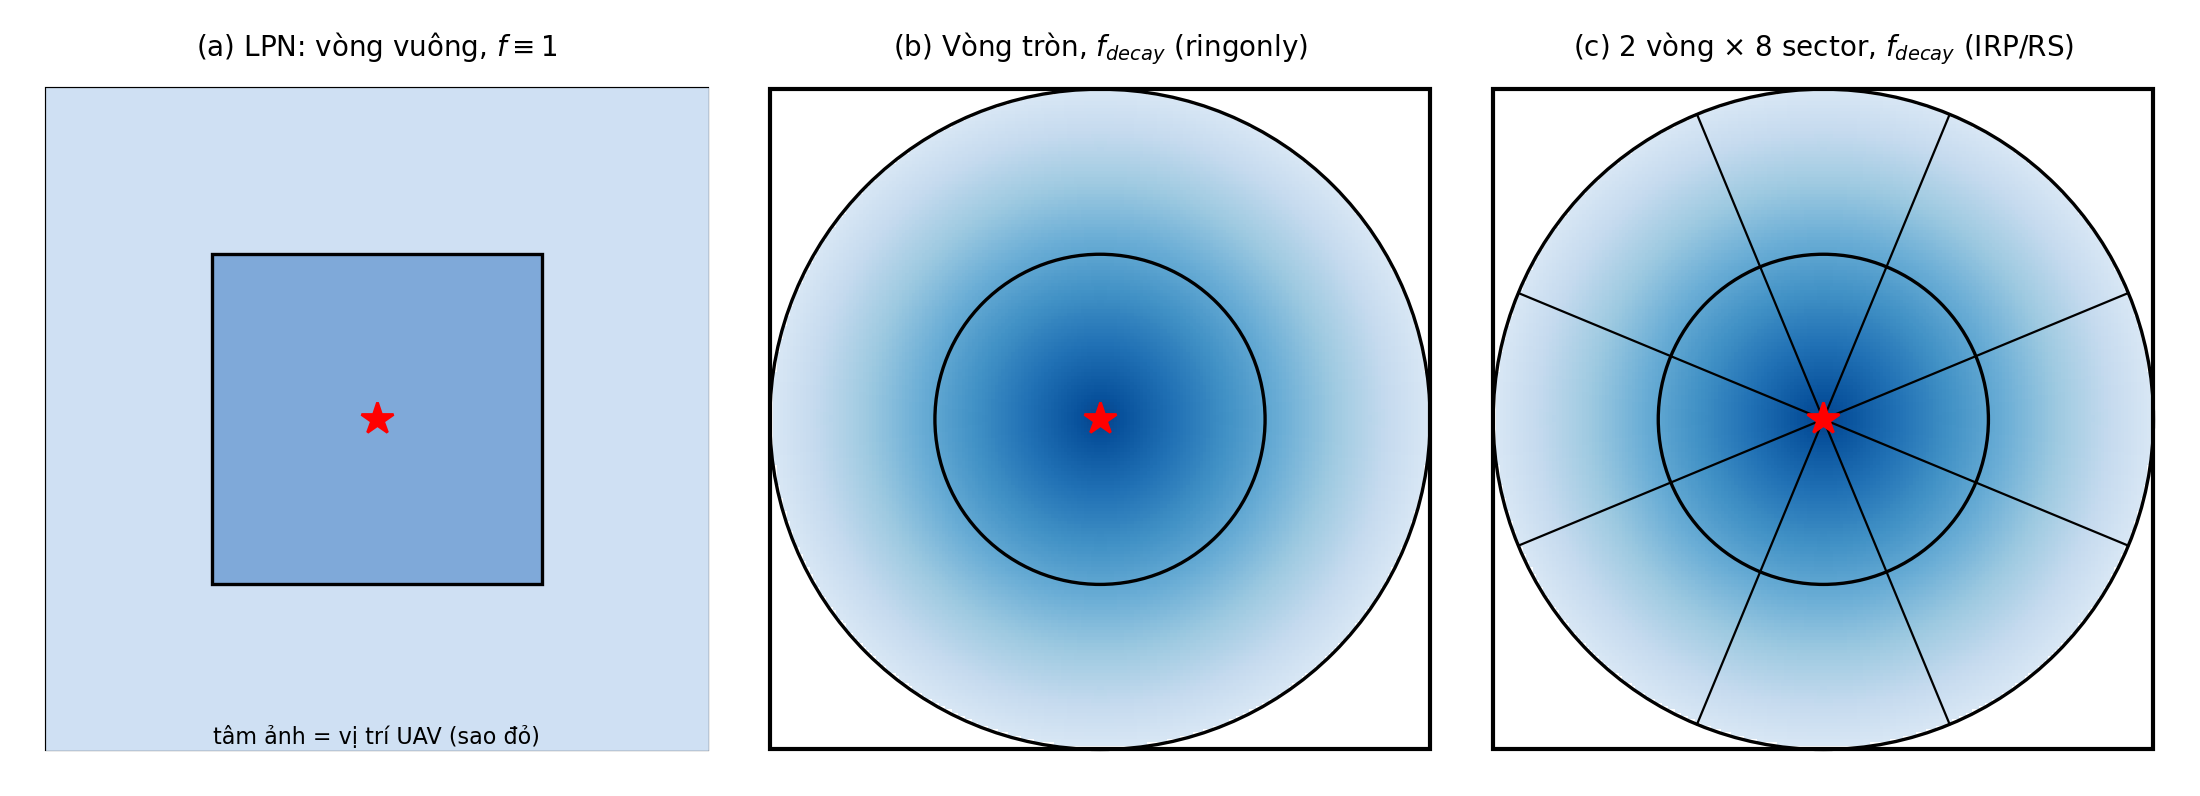
\includegraphics[width=.8\linewidth]{fig1_phanhoach.png}
\caption{Ba cách phân hoạch ảnh. Màu càng đậm thì trọng số càng lớn. Ngôi sao là vị trí UAV.}\label{fig:phanhoach}
\end{figure}

\begin{figure}[H]\centering
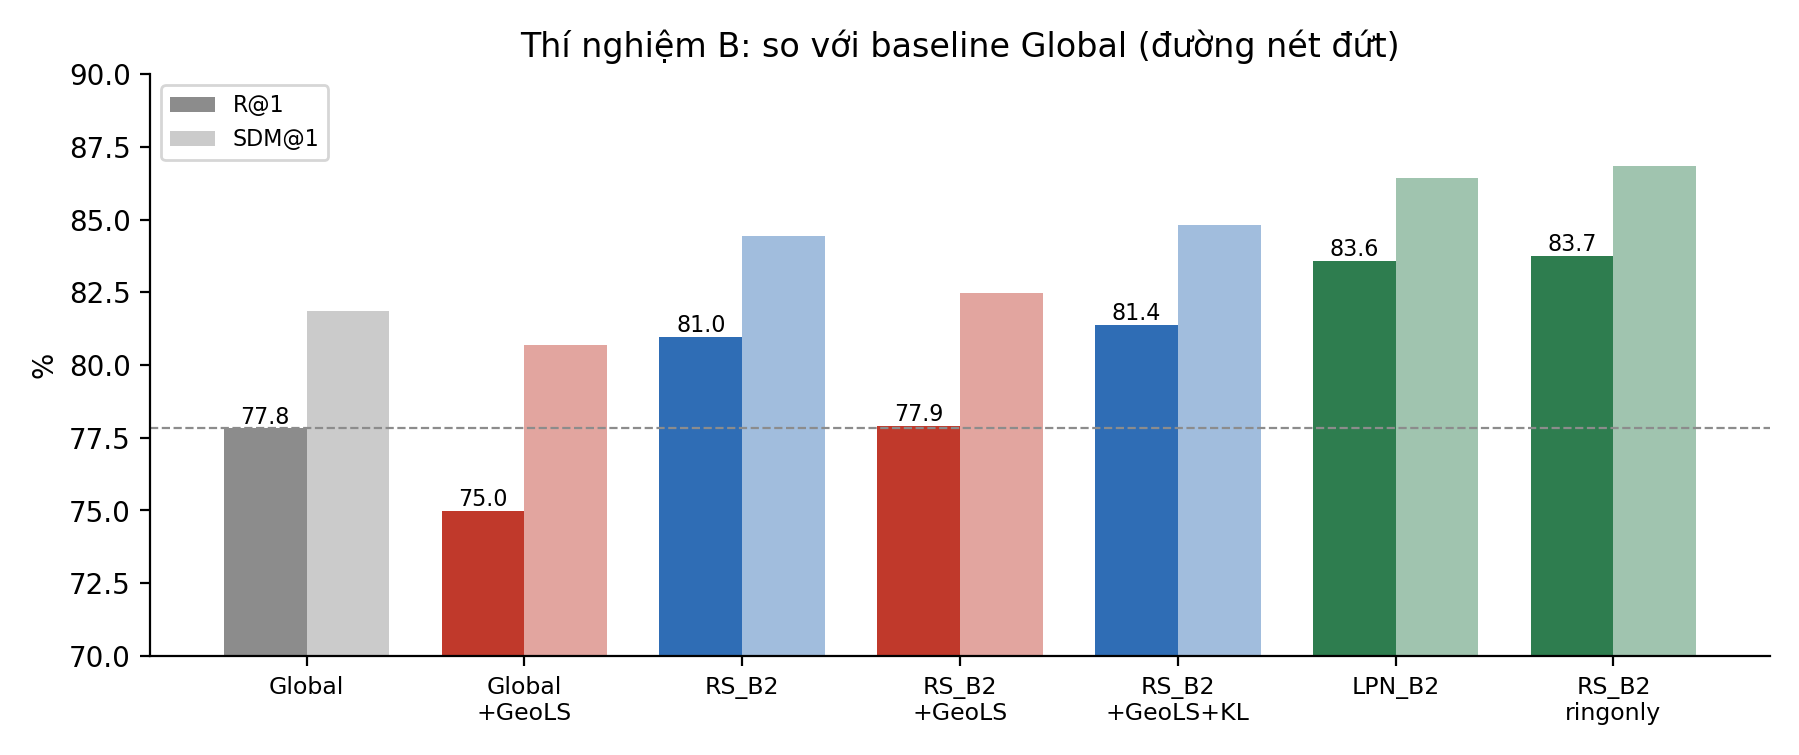
\includegraphics[width=.8\linewidth]{fig2_thinghiemB.png}
\caption{Kết quả thí nghiệm B. Run dùng DINOv2 bị hỏng (20.6\%) nên không đưa vào hình.}\label{fig:B}
\end{figure}

Phân hoạch theo vòng cải thiện rõ (Hình~\ref{fig:B}): từ baseline Global 77.82, LPN đạt 83.57 và vòng tròn có trọng số đạt 83.74. Chênh lệch 0.17 điểm giữa vòng tròn và vòng vuông nhỏ hơn dao động do seed, nên chưa thể kết luận phương án vòng tròn tốt hơn LPN.

Chia thêm 8 cung để bất biến hướng bay lại làm R@1 giảm từ 83.74 xuống 80.95. Ở thí nghiệm A, head IRP (cũng 2 vòng $\times$ 8 cung) đạt 84.73, ngang LPN (84.77). Ở thí nghiệm C, IRP đạt 83.35, cao hơn Global 5.87 điểm. C không có run LPN và IRP dùng learning rate khác baseline, nên chưa tách được phần tăng do phân hoạch vòng với phần do chia cung hay do learning rate.

\begin{figure}[H]\centering
\begin{minipage}{.48\linewidth}\centering
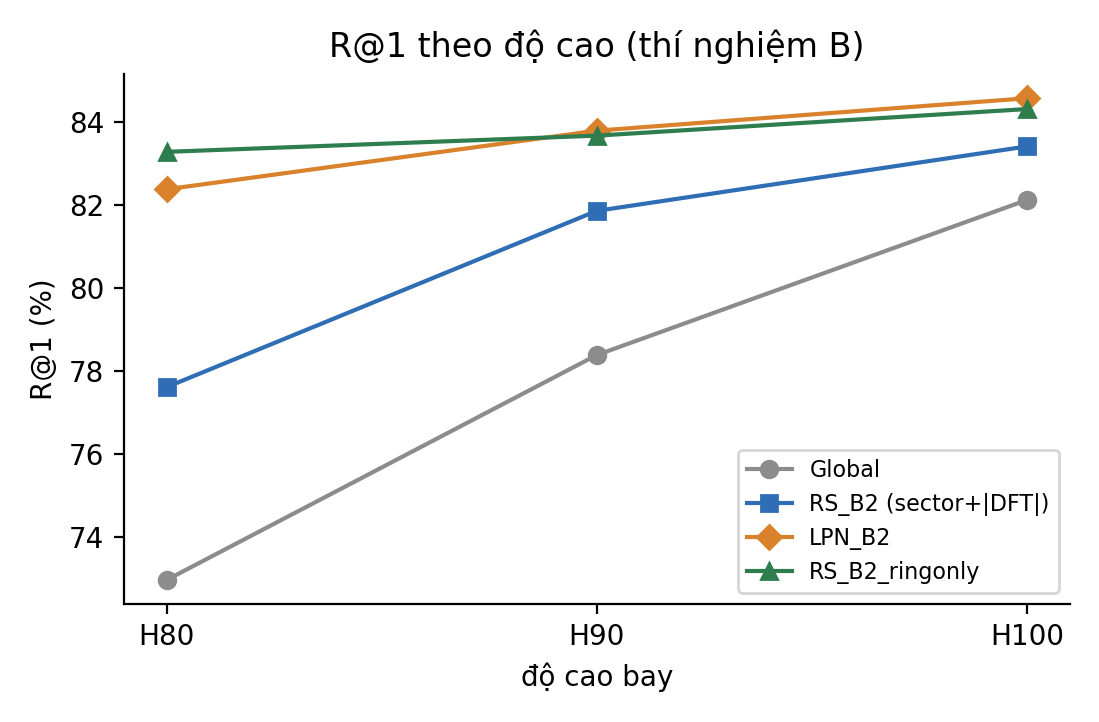
\includegraphics[width=\linewidth]{fig5_docao.png}
\caption{R@1 theo độ cao bay.}\label{fig:docao}
\end{minipage}\hfill
\begin{minipage}{.44\linewidth}\centering
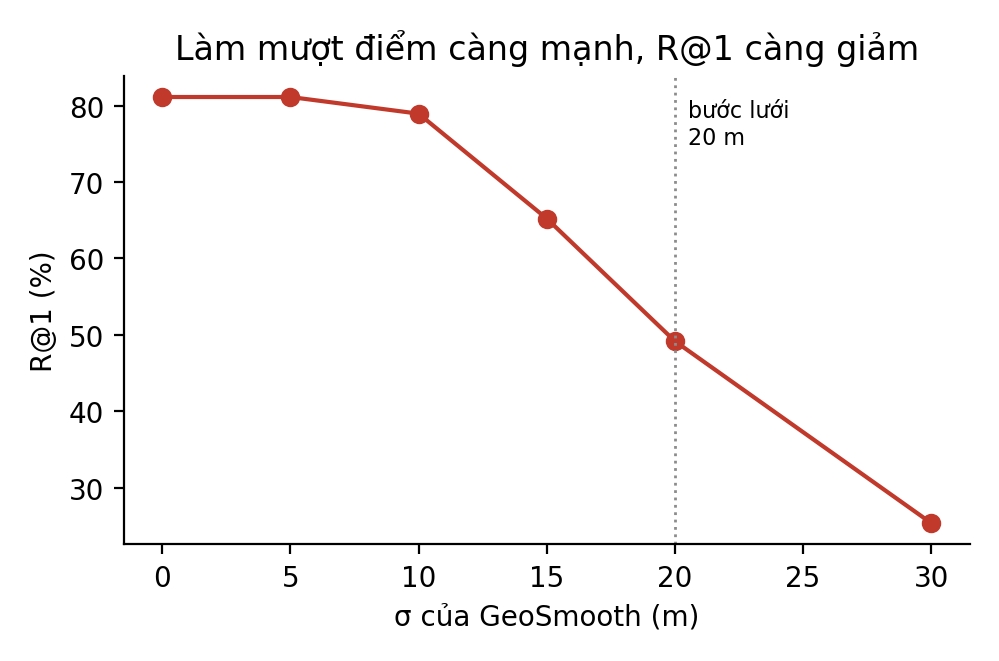
\includegraphics[width=\linewidth]{fig7_sigma.png}
\caption{R@1 theo $\sigma$ của GeoSmooth (mục CT2).}\label{fig:sigma}
\end{minipage}
\end{figure}

Theo độ cao bay (Hình~\ref{fig:docao}), phân hoạch vòng tăng hơn 10 điểm ở 80\,m nhưng chỉ khoảng 2 điểm ở 100\,m. Giả thuyết: ảnh chụp thấp phủ vùng nhỏ hơn, nên thông tin vật thể gần hay xa tâm có ích hơn.

\section{CT2: nhất quán không gian dạng mềm}
Ba phương án đã thử. Ký hiệu $x_c$ là toạ độ (mét) của vị trí $c$, $d_{cc'}=|x_c-x_{c'}|$, và
\[
K^{\sigma}_{cc'}=e^{-d_{cc'}^2/(2\sigma^2)}\,\mathbf 1[d_{cc'}\le3\sigma],\qquad \tilde K^{\sigma}_{cc'}=\frac{K^{\sigma}_{cc'}}{\sum_{c''}K^{\sigma}_{cc''}}.
\]

\emph{A và C, loss thứ tự.} Trong batch (cả ảnh drone và vệ tinh), $u_a$ là đặc trưng đã chuẩn hoá, $d_f(a,b)=\|u_a-u_b\|$, $d_g(a,b)$ là khoảng cách GPS, $A$ là các mẫu có cả láng giềng trong 30\,m lẫn mẫu xa trên 60\,m:
\[
\mathcal L_{LC}=\frac1{|A|}\sum_{a\in A}\operatorname{softplus}\Big(\alpha\big(\max_{0<d_g(a,b)\le30}d_f(a,b)-\min_{d_g(a,b')>60}d_f(a,b')\big)\Big),\qquad\alpha=3.
\]
Loss chỉ ràng buộc thứ tự gần xa, không ràng buộc hằng số Lipschitz. Head nhiều nhánh lấy trung bình $\mathcal L_{LC}$ qua các nhánh; loss tổng là $\mathcal L_{\text{repo}}+\mathcal L_{LC}$. Loss được chạy kèm hai cách lấy mẫu, đều giữ mỗi lớp đúng một lần mỗi epoch:
\begin{itemize}
\item GeoSampler: mỗi lớp đi kèm tối đa 3 láng giềng GPS trong 30\,m;
\item DSS theo CEUSP~\cite{ceusp}: từ epoch 20, mỗi nhóm gồm lớp neo, 1 láng giềng GPS và 2 lớp mô hình đang dễ nhầm nhất, cập nhật mỗi 6 epoch.
\end{itemize}

\emph{B, GeoLS.} Thay nhãn one-hot của lớp $y$ bằng phân phối
\[
T_{y}=(1-\varepsilon)\,e_y+\varepsilon\,\tilde K^{\sigma}_{y,\cdot}\big|_{c\ne y},\qquad \mathcal L_{\text{GeoLS}}=-\sum_c T_{yc}\log p_c,
\]
với $\varepsilon=0.1$, $\sigma=20$\,m, $\tilde K$ chuẩn hoá trên các lớp $c\ne y$; lớp không có láng giềng giữ nhãn cứng.

\emph{B, GeoSmooth.} Lúc test, với $\bar s(q,c)$ là điểm trung bình của 6 ảnh vệ tinh của vị trí $c$,
\[
s'(q,c)=\sum_{c'}\tilde K^{\sigma}_{cc'}\,\bar s(q,c'),
\]
gán cho mọi ảnh của $c$. Trường hợp $\sigma=0$ là loc-fuse ở mục sau.

\begin{figure}[H]\centering
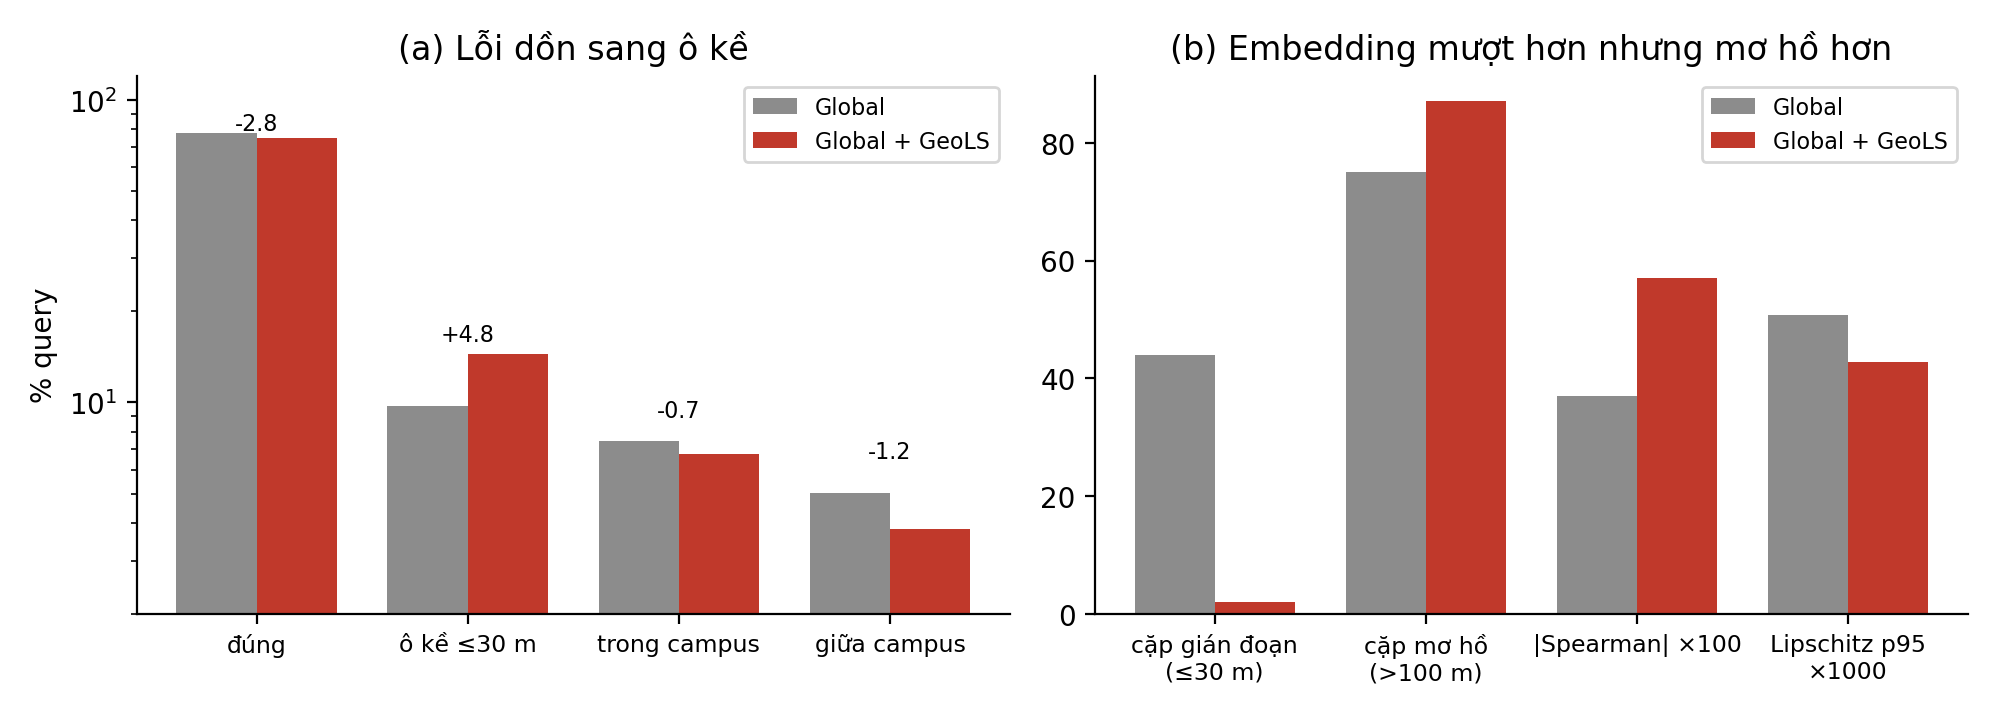
\includegraphics[width=.85\linewidth]{fig6_geols.png}
\caption{Global trước và sau khi thêm GeoLS.}\label{fig:geols}
\end{figure}

GeoLS làm embedding mượt hơn (Hình~\ref{fig:geols}b): số cặp ô kề có đặc trưng khác hẳn nhau giảm từ 44 xuống 2, hằng số Lipschitz đo được ($\hat L$ trong~\eqref{eq:lip}) cũng giảm. Tuy nhiên R@1 giảm 2.8 điểm, do lỗi nhầm sang ô kề tăng từ 9.7\% lên 14.5\% (Hình~\ref{fig:geols}a).

Các ô trong DenseUAV chỉ cách nhau 20\,m trong khi R@1 yêu cầu chọn đúng một ô; embedding càng mượt thì hai ô kề càng khó tách. SDM@1 chỉ giảm 1.2 điểm vì các lỗi mới đều nằm gần vị trí đúng.

GeoSampler + loss tăng 0.56 điểm ở A, nhỏ hơn mức nhiễu nên không được tính là có tác dụng. Ở C, cùng cấu hình đó tăng 2.06 điểm so với Global, vượt nhiễu seed (0.73). Tuy nhiên DSS không có loss tăng 3.17 điểm, còn thêm loss vào DSS lại giảm 0.30 (80.65 xuống 80.35). Ở A, thêm loss vào DSS giảm mạnh hơn: 83.44, thấp hơn DSS 2.45 điểm và thấp hơn baseline LPN 1.33 điểm. Phần tăng ở C vì vậy nhiều khả năng đến từ cách lấy mẫu batch chứ không từ loss. GeoSmooth càng làm mượt mạnh càng giảm (Hình~\ref{fig:sigma}); các giá trị $\sigma$ được chọn trước khi chạy, không chọn theo kết quả test.

\section{Kỹ thuật lúc test}
\begin{figure}[H]\centering
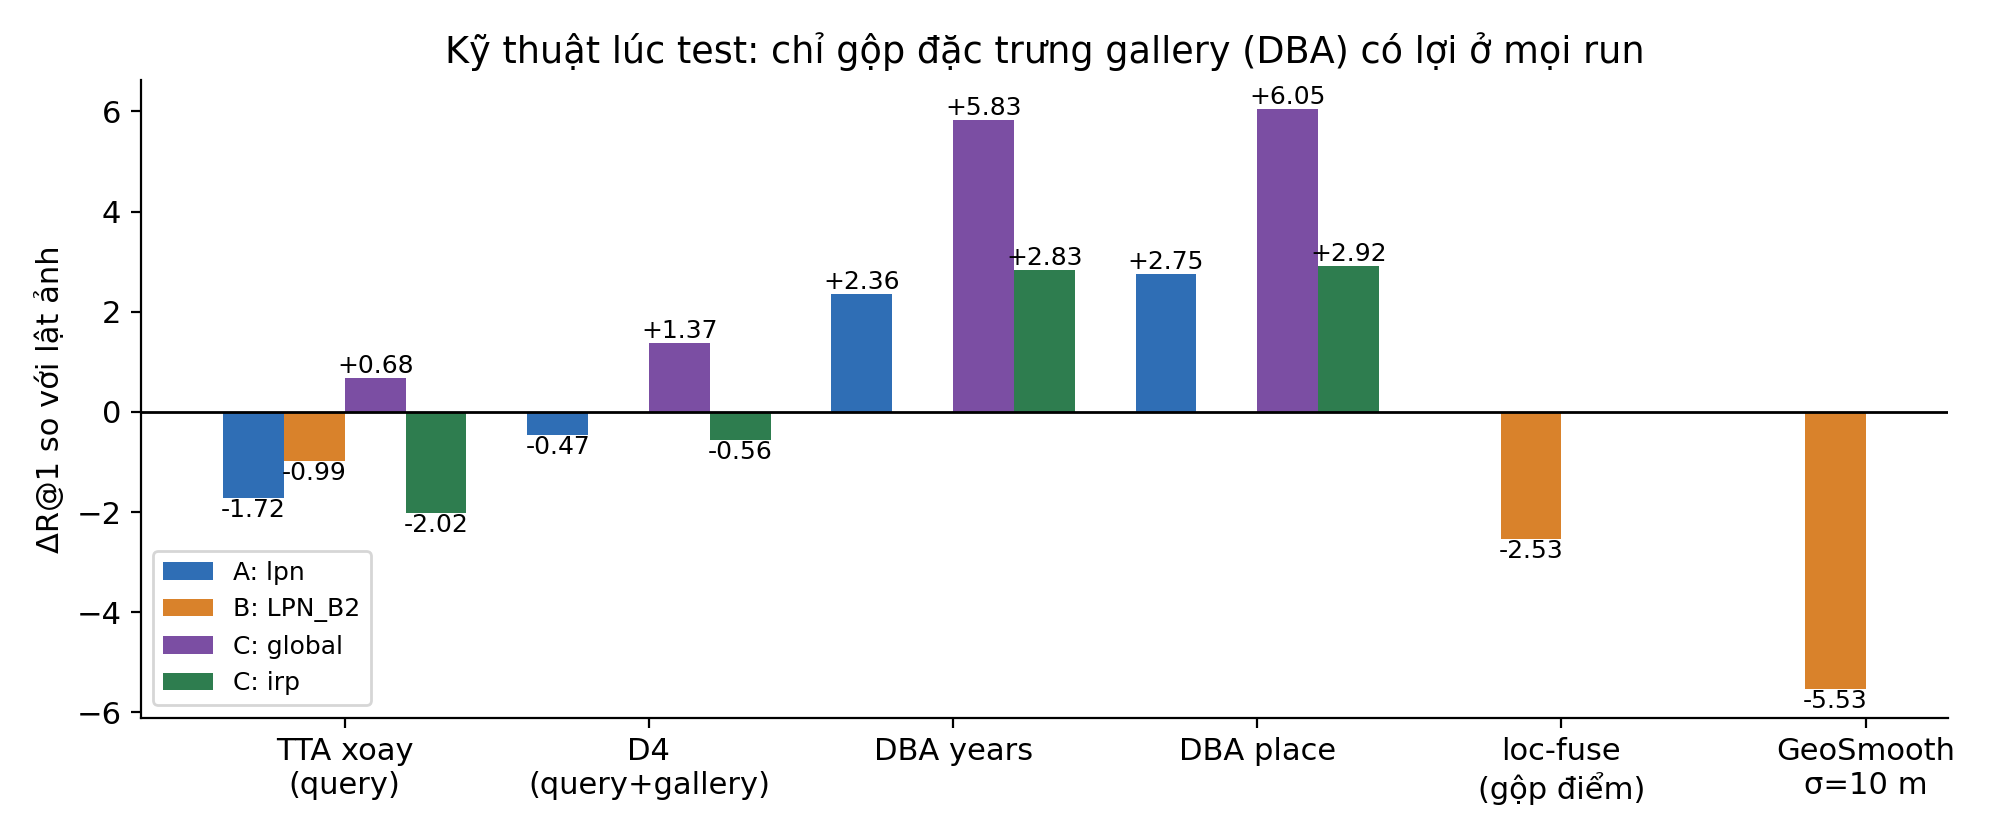
\includegraphics[width=.75\linewidth]{fig4_testtime.png}
\caption{Thay đổi R@1 so với cách lật ảnh mặc định của repo.}\label{fig:tt}
\end{figure}

Gọi $\phi(x)$ là đặc trưng của ảnh $x$, $\bar x$ là ảnh lật ngang, $r$ là phép xoay $90^\circ$ và $\mathrm{norm}$ là chuẩn hoá $L^2$ (từng nhánh rồi cả vector, như \texttt{test.py}). Repo mặc định dùng $\mathrm{norm}(\phi(x)+\phi(\bar x))$. Hai kỹ thuật được thử là
\[
\phi_{D_4}(x)=\mathrm{norm}\Big(\sum_{k=0}^{3}\big(\phi(r^kx)+\phi(r^k\bar x)\big)\Big),\qquad
p_G=\mathrm{norm}\Big(\sum_{g\in G}\phi_{D_4}(g)\Big),
\]
trong đó DBA thay đặc trưng mỗi ảnh vệ tinh bằng $p_G$ của nhóm $G$ chứa nó. \emph{DBA năm} gom 2 ảnh cùng vị trí, cùng mức thu phóng, khác năm chụp; \emph{DBA vị trí} gom cả 6 ảnh. ``D4 + DBA'' trong báo cáo là D4 cho cả drone lẫn vệ tinh cộng DBA năm.

Kết quả các kỹ thuật lúc test (Hình~\ref{fig:tt}):
\begin{itemize}
\item D4 cho ảnh drone: R@1 giảm ở cả 12 run có phân hoạch vòng (6 run ở A, 5 run ở B và IRP ở C). Với head Global ở C, kết quả trái chiều: tăng 0.68 điểm với baseline nhưng giảm 2.10 điểm với ViT-B.
\item DBA: so với cách lật ảnh mặc định, R@1 tăng 2.4--2.9 điểm với head phân hoạch vòng (LPN ở A, IRP ở C) và 5.8--6.1 điểm với Global ở C. Đây là mức tăng lớn nhất trong các kỹ thuật đã thử. DBA chỉ dùng thông tin bản đồ có sẵn (ảnh nào thuộc ô nào) nên áp dụng được khi triển khai thực tế, nhưng khi so sánh với các công trình khác sẽ được báo cáo riêng.
\item Loc-fuse ở B (GeoSmooth với $\sigma=0$: gộp \emph{điểm số} của 6 ảnh thay vì \emph{đặc trưng}) làm kết quả giảm, nhiều khả năng do thiếu bước chuẩn hoá sau khi lấy trung bình. Phần này sẽ được sửa và chạy lại.
\end{itemize}

\begin{figure}[H]\centering
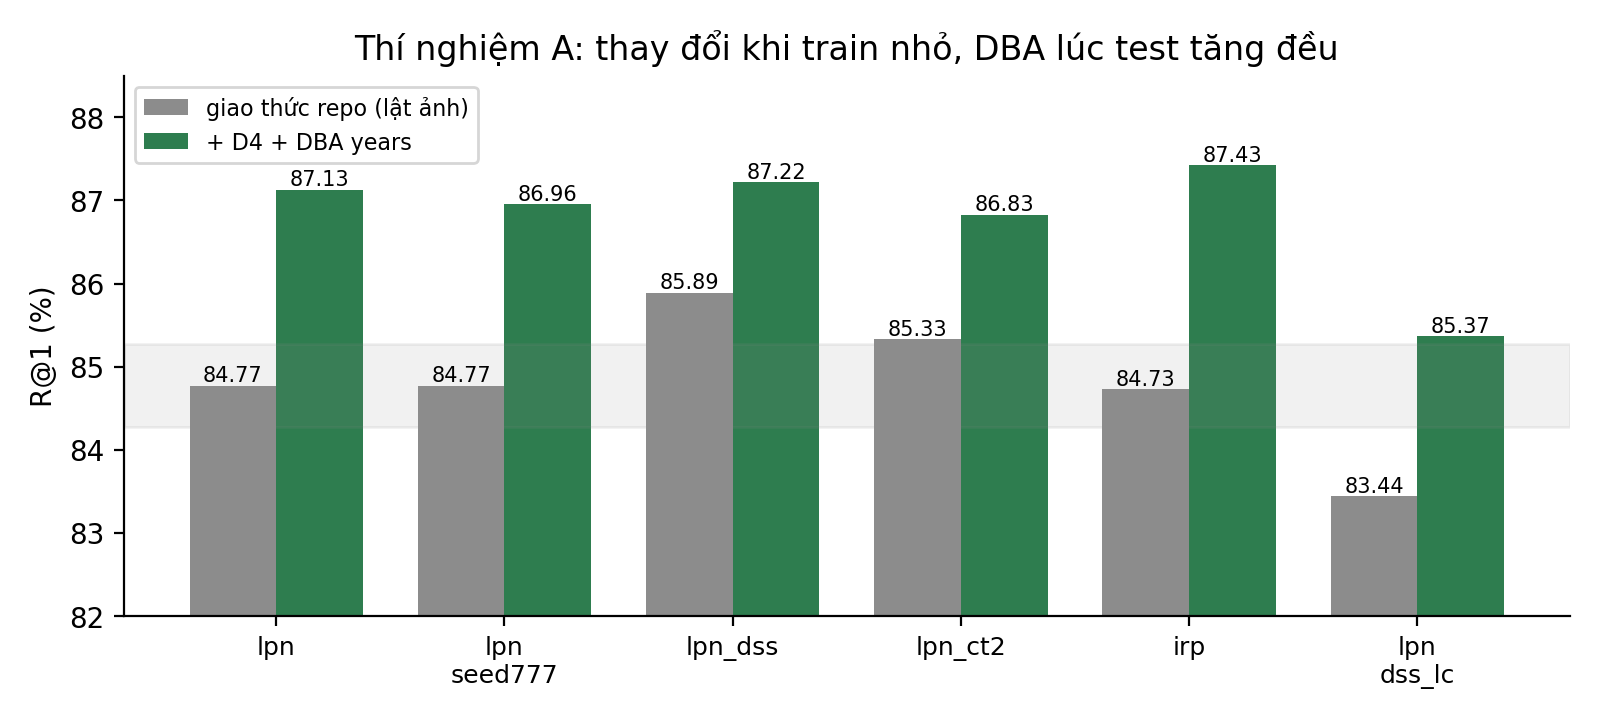
\includegraphics[width=.7\linewidth]{fig3_thinghiemA.png}
\caption{Thí nghiệm A, trước và sau khi thêm D4 + DBA.}\label{fig:A}
\end{figure}

Ở thí nghiệm A (Hình~\ref{fig:A}), thay đổi lúc train có triển vọng nhất là lấy mẫu động DSS theo CEUSP~\cite{ceusp}, tăng 1.12 điểm. Sau khi thêm DBA, các run nằm trong khoảng 0.6 điểm (86.83--87.43), trừ DSS + loss (85.37).

\begin{figure}[H]\centering
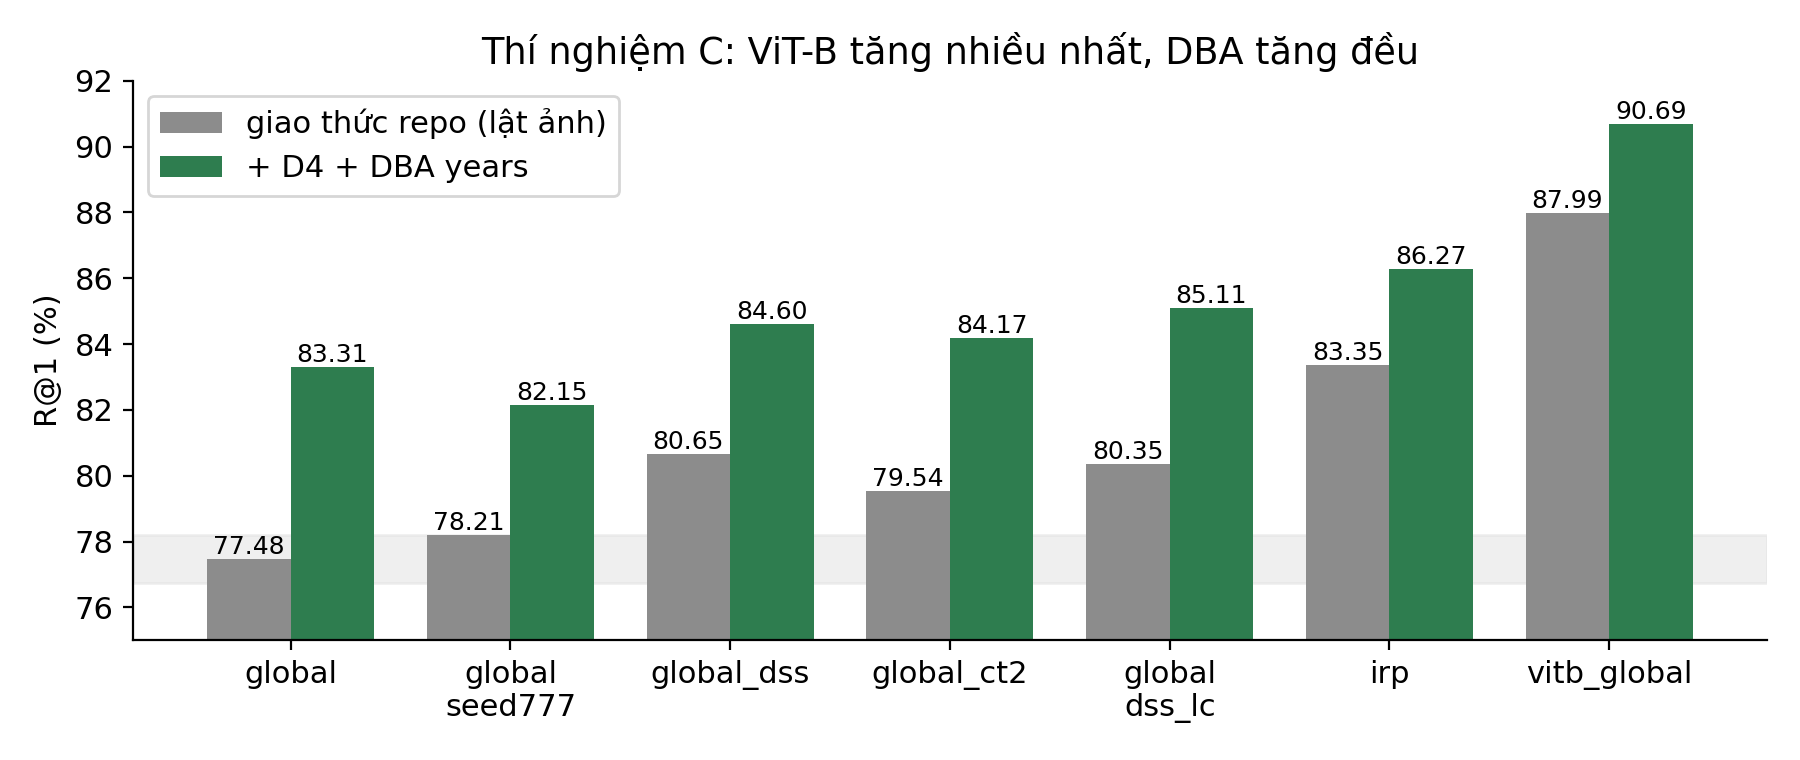
\includegraphics[width=.75\linewidth]{fig8_thinghiemC.png}
\caption{Thí nghiệm C, trước và sau khi thêm D4 + DBA. Dải xám là nhiễu seed của baseline ($\pm$0.73).}\label{fig:C}
\end{figure}

Ở thí nghiệm C (Hình~\ref{fig:C}), DSS tăng 3.17 điểm R@1 so với Global, lớn hơn ở A. D4 cho kết quả trái chiều: tăng 1.37 điểm với Global nhưng giảm với IRP (0.56) và ViT-B (0.69). DBA tăng thêm 3.3--4.5 điểm so với D4 ở mọi run ViT-S và 3.4 điểm với ViT-B. Sau DBA, sai số trung vị của các dự đoán sai ở mọi run đều khoảng 21\,m.

So sánh từng query giữa hai lần chạy baseline với hai seed khác nhau ở A cho thấy khoảng 4\% query đổi trạng thái đúng/sai chỉ do seed. Ở C, đổi seed làm R@1 lệch 0.73 điểm và SDM@1 lệch 0.62 điểm. Cần chạy nhiều seed hơn trước khi kết luận.

\section{CT3: phân tích lỗi}
Campus $\kappa(c)$ của vị trí $c$ là thành phần liên thông của đồ thị nối các vị trí cách nhau không quá 200\,m (A, C) hoặc 100\,m (B). Với top-1 $\hat y$ và vị trí đúng $y$, kết quả thuộc một trong bốn loại:
\[
\text{đúng: }\hat y=y;\quad
\text{ô kề: }\hat y\ne y,\ d_{y\hat y}\le30\,\text{m};\quad
\text{trong campus: }d_{y\hat y}>30\,\text{m},\ \kappa(\hat y)=\kappa(y);\quad
\text{khác campus: }\kappa(\hat y)\ne\kappa(y).
\]
Ở A, C, dự đoán rơi vào vị trí của tập train cũng tính là khác campus. Hai loại cuối gọi chung là lỗi xa.

Mỗi vị trí có prototype $P_c=\mathrm{norm}\big(\sum_{g\in c}\phi(g)\big)$ từ các ảnh vệ tinh; $u_q$ là đặc trưng query đã chuẩn hoá. Lỗi xa là \emph{cặp mơ hồ} (hai vị trí vốn giống nhau) nếu ở A, C
\[
1-\cos(P_y,P_{\hat y})<\operatorname*{median}_{q'\in Q}\big(1-\cos(u_{q'},P_{y(q')})\big),
\]
và là \emph{lệch miền} nếu ngược lại. Ở B, cặp vị trí $(c,c')$ là mơ hồ nếu $d_{cc'}>100$\,m và $\cos(P_c,P_{c'})\ge\tau=\operatorname{median}_{q}\cos(u_q,P_{y(q)})$.

\begin{figure}[H]\centering
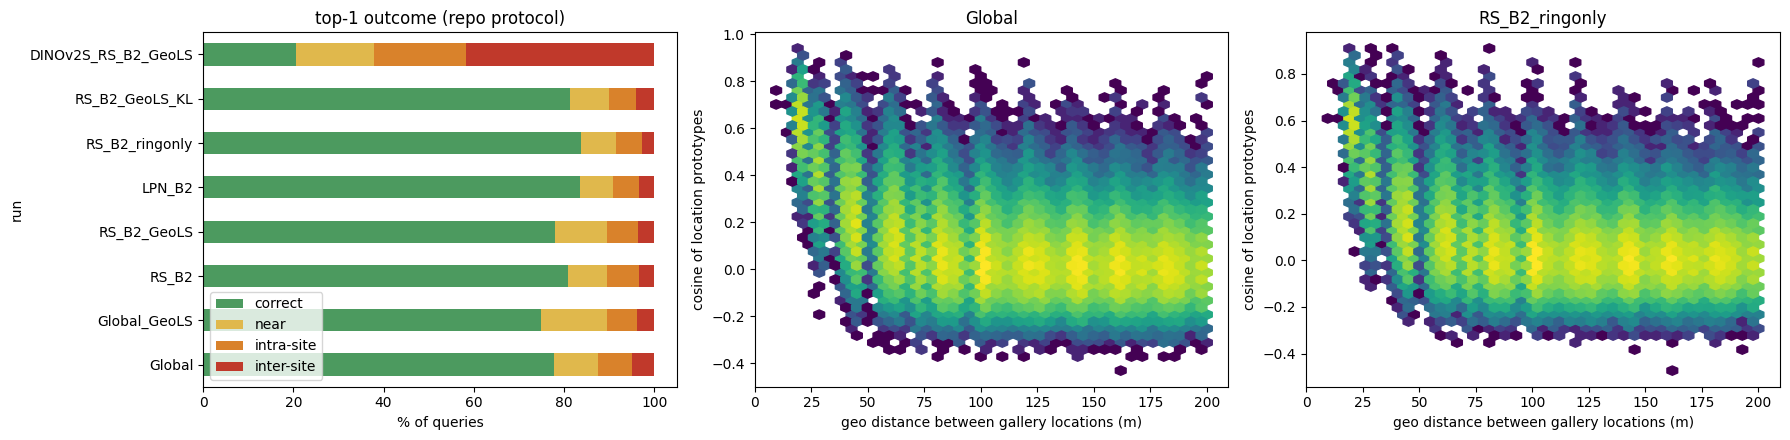
\includegraphics[width=\linewidth]{nb_baseline06v3_c21_0.png}
\caption{Thí nghiệm B. Trái: tỉ lệ từng loại kết quả của mỗi run (xanh lá: đúng; vàng: ô kề; cam: trong campus; đỏ: khác campus). Giữa và phải: cosine giữa đặc trưng của hai ô vệ tinh cùng campus theo khoảng cách, với Global và vòng tròn.}\label{fig:err}
\end{figure}

\begin{figure}[H]\centering
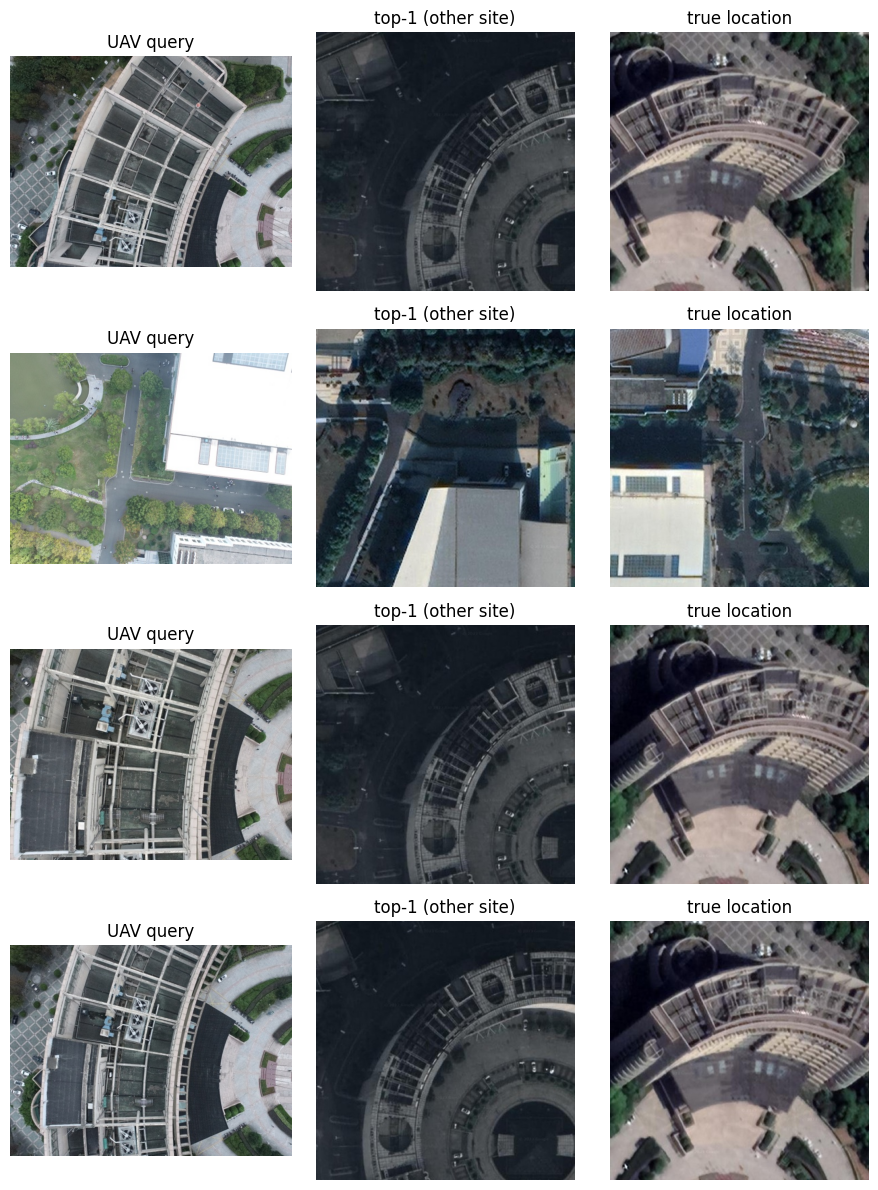
\includegraphics[width=.42\linewidth]{nb_baseline06v3_c21_1.png}
\caption{Bốn lỗi nhầm campus có độ tin cậy cao nhất (run vòng tròn, có xoay ảnh lúc test và GeoSmooth $\sigma=10$\,m). Trái: ảnh drone; giữa: ảnh được chọn; phải: vị trí đúng.}\label{fig:sai}
\end{figure}

Lỗi phổ biến nhất là nhầm sang ô kề. Với baseline LPN ở A, trong 15.2\% lỗi có 6.6\% là ô kề; thêm DBA làm sai số trung vị của các dự đoán sai giảm từ 43\,m xuống 21\,m. Trong các lỗi xa ở A, khoảng một phần ba là cặp mơ hồ, phần còn lại là lệch miền.

\begin{table}[H]\centering\small
\caption{Tỉ lệ từng loại kết quả (\% query), giao thức của repo. Ở C, số được tính lại từ đặc trưng; với IRP, R@1 tính lại là 83.44, lệch 0.09 so với 83.35 trong \texttt{results.txt}.}\label{tab:loi}
\begin{tabular}{@{}llrrrr@{}}\toprule
TN & Run & Đúng & Ô kề & Trong campus & Khác campus\\\midrule
B & Global & 77.82 & 9.70 & 7.46 & 5.02\\
B & Vòng tròn & 83.74 & 7.68 & 5.83 & 2.75\\\midrule
C & Global & 77.48 & 11.33 & 6.86 & 4.34\\
C & IRP & 83.44 & 6.65 & 6.39 & 3.52\\
C & ViT-B & 87.99 & 5.83 & 4.12 & 2.06\\\bottomrule
\end{tabular}
\end{table}

Thí nghiệm B cho kết quả tương tự (Hình~\ref{fig:err}, trái; Bảng~\ref{tab:loi}). Phân hoạch vòng giảm cả ba loại lỗi, mạnh nhất là lỗi khác campus (gần một nửa). Xoay ảnh lúc test giảm thêm lỗi khác campus (2.75 xuống 2.36) nhưng tăng lỗi ô kề (7.68 lên 9.57), tức là giúp xác định đúng khu vực nhưng làm mất chi tiết để phân biệt hai ô sát nhau.

Thí nghiệm C (giao thức của repo, chưa dùng D4 và DBA) cho cùng xu hướng (Bảng~\ref{tab:loi}). Khác với B, phân hoạch vòng ở C (IRP) chủ yếu giảm lỗi ô kề (11.33 xuống 6.65), lỗi khác campus chỉ giảm 0.82 điểm. ViT-B giảm cả ba loại và có lỗi khác campus thấp nhất trong mọi run (2.06\%). Tỉ lệ cặp mơ hồ trong các lỗi xa là 27--40\% tuỳ run, khớp với A: phần lớn lỗi xa do lệch miền.

Trên hexbin của thí nghiệm B, cosine giữa hai ô cách nhau 20\,m phân tán rộng, khoảng 0.4 đến 0.9; từ khoảng 75\,m trở đi phần lớn các cặp có cosine quanh 0. Đặc trưng đã tách được các ô xa, khó khăn nằm ở các ô trong bán kính vài chục mét. Trong Bảng~\ref{tab:hexbin}, cặp ô kề \emph{khác hẳn nhau} nếu $\cos(P_c,P_{c'})$ không vượt trung vị cosine của các cặp cùng campus cách 60--100\,m; Spearman tính trên các cặp cùng campus cách không quá 200\,m. Hằng số Lipschitz thực nghiệm là
\begin{equation}\label{eq:lip}
\hat L=\operatorname*{median}_{d_{cc'}\le30\,\text{m}}\frac{\|P_c-P_{c'}\|}{d_{cc'}}\quad(1/\text{m}).
\end{equation}
Phân hoạch vòng giảm mạnh số cặp ô xa có đặc trưng giống nhau nhưng tăng số cặp ô kề có đặc trưng khác hẳn nhau (Bảng~\ref{tab:hexbin}); tương quan giữa khoảng cách và cosine gần như không đổi.

\begin{table}[H]\centering\small
\caption{Cấu trúc không gian của embedding, thí nghiệm B.}\label{tab:hexbin}
\begin{tabular}{@{}lrr@{}}\toprule
& Global & Vòng tròn\\\midrule
Cặp ô cách trên 100\,m có cosine vượt $\tau$ & 75 & 24\\
Cặp ô kề có đặc trưng khác hẳn nhau & 44 & 73\\
Spearman (khoảng cách, cosine) & $-0.37$ & $-0.33$\\\bottomrule
\end{tabular}
\end{table}

Trong Hình~\ref{fig:sai}, mô hình đều chọn nhầm một toà nhà cong rất giống toà nhà thật, và ảnh vệ tinh bị chọn tối hơn (có thể khác năm hoặc giờ chụp). Hàng 1, 3 và 4 là cùng một vị trí ở ba độ cao, nên bốn lỗi thực chất đến từ hai vị trí. Ở hàng 2, ảnh bị chọn cũng có một mái nhà trắng lớn giống ảnh drone. Ảnh drone trong các ví dụ này dường như bị xoay so với ảnh vệ tinh, liên quan đến vấn đề bất biến xoay ở mục sau.

\section{Đối chiếu với bài shape vector}\label{sec:doichieu}

\subsection{Công thức}
Head đã cài đặt chưa đúng công thức của bài. Công thức (3.3) là
\[
w_i(x^*)=\int_\Omega f_{x^*}\,\chi_{V(x^*)\cap U_i(x^*)}\,dm,
\]
tức tích phân trọng số trên phần \emph{nhìn thấy được} của ô, chỉ chứa thông tin hình học và không chuẩn hoá. Cài đặt hiện tại thay $\chi_V$ bằng đặc trưng $\varphi$ của ViT và chia thêm cho $\int f$. Khi $\varphi=\chi_V$, head cho đúng $w_i(x^*)/\int_{U_i}f\,dm$; khi $f\equiv1$, head trùng với trung bình ô trong Định nghĩa 5.2. Do đó trong paper nên gọi đây là ``mở rộng'' thay vì ``áp dụng'' công thức của bài.

\subsection{Trích dẫn}
Notebook ghi nhầm ``Def.~3.3''. Bài không có Định nghĩa 3.3: (3.3) là số hiệu phương trình, còn số 3.3 trong dãy định lý là Mệnh đề 3.3 (tính nửa liên tục dưới của $W$).

\subsection{Bất biến xoay}
Phần Limitations của bài nêu rằng các cung cố định theo hướng bản đồ, nên ảnh quan sát cần được xoay theo hướng bay trước. Phần Future work gợi ý hai cách đạt bất biến xoay: căn theo hướng bay, hoặc dùng tổ hợp bất biến kiểu moment Hu~\cite{hu1962}. Cách thứ hai (chia cung rồi lấy $|\mathrm{DFT}|$) đã thử: ở B, R@1 giảm 2.79 điểm so với vòng tròn không chia cung; ở A, IRP chỉ ngang LPN. Hai nguyên nhân khả dĩ:
\begin{itemize}
\item phần lớn ảnh drone vốn gần đúng hướng bản đồ, nên bỏ thông tin hướng là bỏ thông tin hữu ích;
\item $|\mathrm{DFT}|$ làm mất quá nhiều thông tin.
\end{itemize}
Cần khảo sát phân bố hướng bay trong dữ liệu để phân biệt hai khả năng này.

\subsection{Tinh phân hoạch}
Định lý 5.4: với $R_Ng$ là trung bình ô (Định nghĩa 5.2) trên phân hoạch có đường kính ô lớn nhất $\delta_N\to0$, ta có $\|R_Ng-g\|_{L^p}\to0$ với mọi $g\in L^p(U(x^*))$, $1\le p<\infty$. Hệ quả 5.5: nếu $g_1\ne g_2$ trên tập có độ đo dương thì $W^N(g_1)\ne W^N(g_2)$ với mọi $N$ đủ lớn. Tức là phân hoạch càng mịn thì phân biệt càng tốt; Bảng 2 của bài cho thấy số ứng viên giảm từ 4 xuống 1. Trong thí nghiệm B, 8 cung lại thua 1 cung (80.95 so với 83.74). A và C không có cặp run chỉ khác nhau ở số cung, nên mức tăng của IRP ở C không dùng để kiểm tra định lý được. Hai kết quả này không mâu thuẫn vì:
\begin{itemize}
\item Hệ quả 5.5 xét toàn bộ vector, còn cài đặt chỉ giữ $|\mathrm{DFT}|$ (mất pha);
\item đặc trưng ở đây là học được, không cố định như trong định lý;
\item mỗi patch đã là 16\,px, chia nhỏ hơn không thêm thông tin.
\end{itemize}
Dự đoán của định lý do đó chưa được kiểm chứng trên DenseUAV.

\subsection{Trọng số $f$}
Ví dụ 4.1 cho thấy $f_{\mathrm{decay}}$ phân biệt được hai cấu hình mà $f\equiv1$ không phân biệt được. Chưa có run nào so sánh $f_{\mathrm{decay}}$ với $f\equiv1$ trên vòng tròn, nên tác dụng của trọng số trên DenseUAV chưa được xác định. Báo cáo rà soát giả thiết (\texttt{contrib/dong\_gop\_shape\_vector.tex}) đề xuất thêm trọng số bậc thang $f_{\mathrm{step}}=\chi_{B(0,13R/16)}$: trong Ví dụ 4.1, nó tách hai cấu hình với khoảng cách gấp 3.85 lần $f_{\mathrm{decay}}$, nên có thể đưa vào cùng thí nghiệm.

\subsection{Lipschitz}
Mệnh đề 3.7: nếu $f$ Lipschitz và $m\big(E_i(y)\triangle E_i(z)\big)\le M_i|y-z|$ với $E_i=V\cap U_i$, thì
\[
\|W(y)-W(z)\|_1\le\Big(N\,\mathrm{Lip}(f)\,m(U)+\|f\|_\infty\sum_{i=1}^N M_i\Big)|y-z|.
\]
Đây là tính chất của descriptor, bài không đề xuất dùng làm mục tiêu huấn luyện. $\hat L$ trong~\eqref{eq:lip} là phiên bản thực nghiệm của hằng số này; kết quả CT2 cho thấy ép embedding học được mượt hơn làm mất khả năng phân biệt các ô kề.

\section{Hạn chế}
\begin{itemize}
\item Mỗi cấu hình mới chạy một seed. Nhiễu seed của baseline đo ở C là 0.73 điểm R@1, nên chênh lệch dưới khoảng 1 điểm chưa đáng tin.
\item Các baseline thấp hơn lần chạy trước với ảnh gốc khoảng 1.3--2.0 điểm, chưa rõ do thu nhỏ ảnh hay do nhiễu.
\item DINOv2 hỏng cả ba lần (4.8\%, 20.6\% và 3.26\%), nhiều khả năng do learning rate của SGD không phù hợp với backbone này.
\item ViT-B mới chạy với head Global và tốn khoảng 4 lần MACs so với ViT-S.
\item D4 cho kết quả trái chiều giữa các run, nên cấu hình test cuối cần chọn riêng theo từng mô hình.
\end{itemize}

\section{Hướng tiếp theo}\label{sec:huongdi}
Mô hình hiện tại đã xác định đúng khu vực khá tốt (lỗi khác campus còn 2.75\% với vòng tròn ở B và 2.06\% với ViT-B ở C); phần lớn lỗi còn lại là nhầm ô cách vài chục mét. Trọng tâm tiếp theo vì vậy là phân biệt các ô gần nhau. Các hướng dưới đây xếp theo thứ tự ưu tiên.

\subsection{Tìm kiếm hai tầng với shape vector ở tầng sau}
Tầng 1 dùng mô hình tốt nhất hiện có (ViT-B với DBA; với ViT-S là vòng tròn có xoay ảnh lúc test vì giảm lỗi khác campus) để lấy ô top-1 và các ô lân cận trong bán kính khoảng 50\,m. Tầng 2 xếp hạng lại các ô ứng viên bằng vector ring$\times$sector đầy đủ, giữ pha (không dùng $|\mathrm{DFT}|$) và không xoay ảnh.

Lý do: lỗi ô kề chiếm tỉ lệ lớn nhất (với ViT-B, 5.83\% so với 6.18\% của hai loại lỗi xa cộng lại); các ô xa đã tách được; xoay ảnh giúp xác định khu vực nhưng hại khả năng phân biệt ô sát nhau, nên tách hai tầng dùng được cả hai mặt. Định lý 5.4 và Hệ quả 5.5 cũng mô tả đúng bài toán của tầng 2, gần với ý của bài hơn so với nhúng descriptor vào embedding toàn cục.

Trước khi huấn luyện, đặc trưng đã lưu sẽ được dùng để đếm số query có ô đúng nằm trong bán kính 50\,m quanh top-1. Con số này là cận trên mức tăng của tầng 2; nếu nhỏ thì dừng hướng này.

\subsection{Hướng bay của ảnh drone}
Tầng 2 giữ pha nên phụ thuộc hướng ảnh. Cần khảo sát phân bố hướng bay trong DenseUAV: nếu phần lớn ảnh gần đúng hướng bản đồ thì dùng trực tiếp, nếu không thì căn ảnh theo hướng bay như phần Limitations của bài. Kết quả này cũng giúp giải thích vì sao $|\mathrm{DFT}|$ làm kết quả giảm.

\subsection{Giảm lỗi khác campus}
Lỗi khác campus tuy ít nhưng có sai số lớn nhất. Hình~\ref{fig:sai} gợi ý hai cách. Thứ nhất, dùng các cặp ô khác campus có kiến trúc giống nhau (như toà nhà cong) làm hard negative khi train, bắt đầu từ 24 cặp ô cách nhau trên 100\,m có cosine vượt ngưỡng $\tau$. Thứ hai, ảnh bị chọn nhầm thường tối hơn, nên thử thêm augmentation độ sáng và độ tương phản cho ảnh vệ tinh.

\subsection{CT2}
Làm mượt đẩy các ô gần nhau lại sát hơn, đúng chỗ mô hình đang yếu, nên tạm dừng với mục tiêu R@1. Phần giữ lại là lấy mẫu theo láng giềng (GeoSampler, DSS). Nếu tiếp tục, nên đánh giá bằng SDM@1 hoặc MA@20m.

\subsection{Thí nghiệm bổ sung}
\begin{enumerate}
\item Chạy 3 seed cho LPN, DSS, IRP và vòng tròn để xác định ngưỡng chênh lệch đáng tin.
\item So sánh $f_{\mathrm{decay}}$, $f\equiv1$ và $f_{\mathrm{step}}$ trên vòng tròn.
\item Chạy với số vòng 2, 3, 4 và số cung 1, 4, 8, giữ toàn bộ các ô (không dùng $|\mathrm{DFT}|$), để kiểm tra Định lý 5.4. Việc này dùng chung code với tầng 2.
\item Chạy ViT-B với phân hoạch vòng và DSS, vì backbone cho mức tăng lớn nhất còn các thay đổi khác mới chỉ thử trên ViT-S.
\item Ở cấu hình C, chạy LPN và IRP với cùng learning rate để tách phần tăng do phân hoạch vòng, do chia cung và do learning rate.
\item Tìm nguyên nhân DINOv2 hỏng cả ba lần, bắt đầu từ learning rate và optimizer.
\item Sửa loc-fuse và chạy lại. Hiện loc-fuse làm lỗi khác campus tăng gấp đôi (2.36 lên 6.01), nhiều khả năng do lỗi cài đặt.
\end{enumerate}

\begin{thebibliography}{9}\small
\bibitem{huu2026} P.~T.~Huu, P.~T.~An, D.~X.~Vinh, A.-D.~Tran, \emph{Lebesgue integral-based shape vector descriptors with applications to GPS-denied UAV localization}, bản thảo, 2026.
\bibitem{dai2024} M.~Dai, E.~Zheng, Z.~Feng, L.~Qi, J.~Zhuang, W.~Yang, Vision-based UAV self-positioning in low-altitude urban environments, \emph{IEEE Trans.\ Image Process.} 33 (2024) 493--508.
\bibitem{ceusp} CEUSP, arXiv:2502.11408, 2025.
\bibitem{hu1962} M.-K.~Hu, Visual pattern recognition by moment invariants, \emph{IRE Trans.\ Inf.\ Theory} 8(2) (1962) 179--187.
\end{thebibliography}
\end{document}
